\chapter{Project Definition}
The purpose of this Senior Thesis Project is to create a \gls{cnc} interface, capable of receiving standardized G-code through \gls{tcpip}, processing the G-code, and driving motors and \gls{gpio} according to the G-code. 

\section{Project Need}
The modern \gls{cnc} interface is limited to utilization of a full computer system, in combination with a motor driver platform to for complete functional control.
This setup can cost upwards of \$500, depending on the quality and system specifications.
It is the goal of this project to encapsulate these hardware and software requirements completely within a system costing less than \$100.
This will bring the \gls{cnc} interface to a price point comparable with tbat of the modern printer. 

\section{Existing Solutions}
\gls{cnc} system requirments currently rely upon complex computer-driver interfaces to control the machine.
The system requires a complete software package operating from a PC to manipulate an entirely separate set of motor drives running the machine.
While this may be practical for commercial and industrial applications, many of the features provided by this system will not be utilized by the average consumer.

\section{Existing Solutions Improvement}
It is the goal of this project to encapsulate these hardware and software requirements completely within a system costing less than \$100.
In combination of the basic functions provided by the PC with the root functionality of the motor driver unit, the system as a whole can be greatly simplified.
The addition of a Web-Interface will allow for users to operate the \gls{cnc} remotely.
This will bring system functionality to a level on par with the modern printer.

\section{Project Scope}
The \gls{cnc} interface will be configurable to operate on different mechanical systems. 

The mechanical requirements and the human-machine interfacing for the project have been eliminated.
The scope now only includes the software for the G-code interpretation, its upload interface, the master controller, the motor controller and the motor driver board.
The G-code interpretation software will have a G-code file as an input and then output motor driver commands from the master controller to the motor controller.
The motor controller will then send out the driver signals to the motor driver board. 
The motor driver board will take the command outputs from the motor controller and then drive the motors. 
There will also be 16 \gls{gpio} pins, an emergency stop switch, and home switches for the motors. 

\section{Objective Tree}
The following objective tree outlines the requirements for having a functioning \gls{cnc} interface for this Senior Thesis Project.
Safety is the most important objective in this project since the \gls{cnc} interface will control moving components, although these moving components are outside the scope of this report.

Thermal Monitoring was weighted as most important because it is a safety feature.
The Motor Driver is a second priority because it is the main functionality.
The Motor Control and G-Code Interpreter were decided to be equally important by using Piecewise Comparisons.
Motor Control relates to the motor accuracy.
G-Code Interpretation is the software interface that will allow a file to be uploaded and sent through TCP/IP.
The Power Supply range is least important because the unit can ship with a standard, tested power supply.

\begin{figure}[H]
\centering
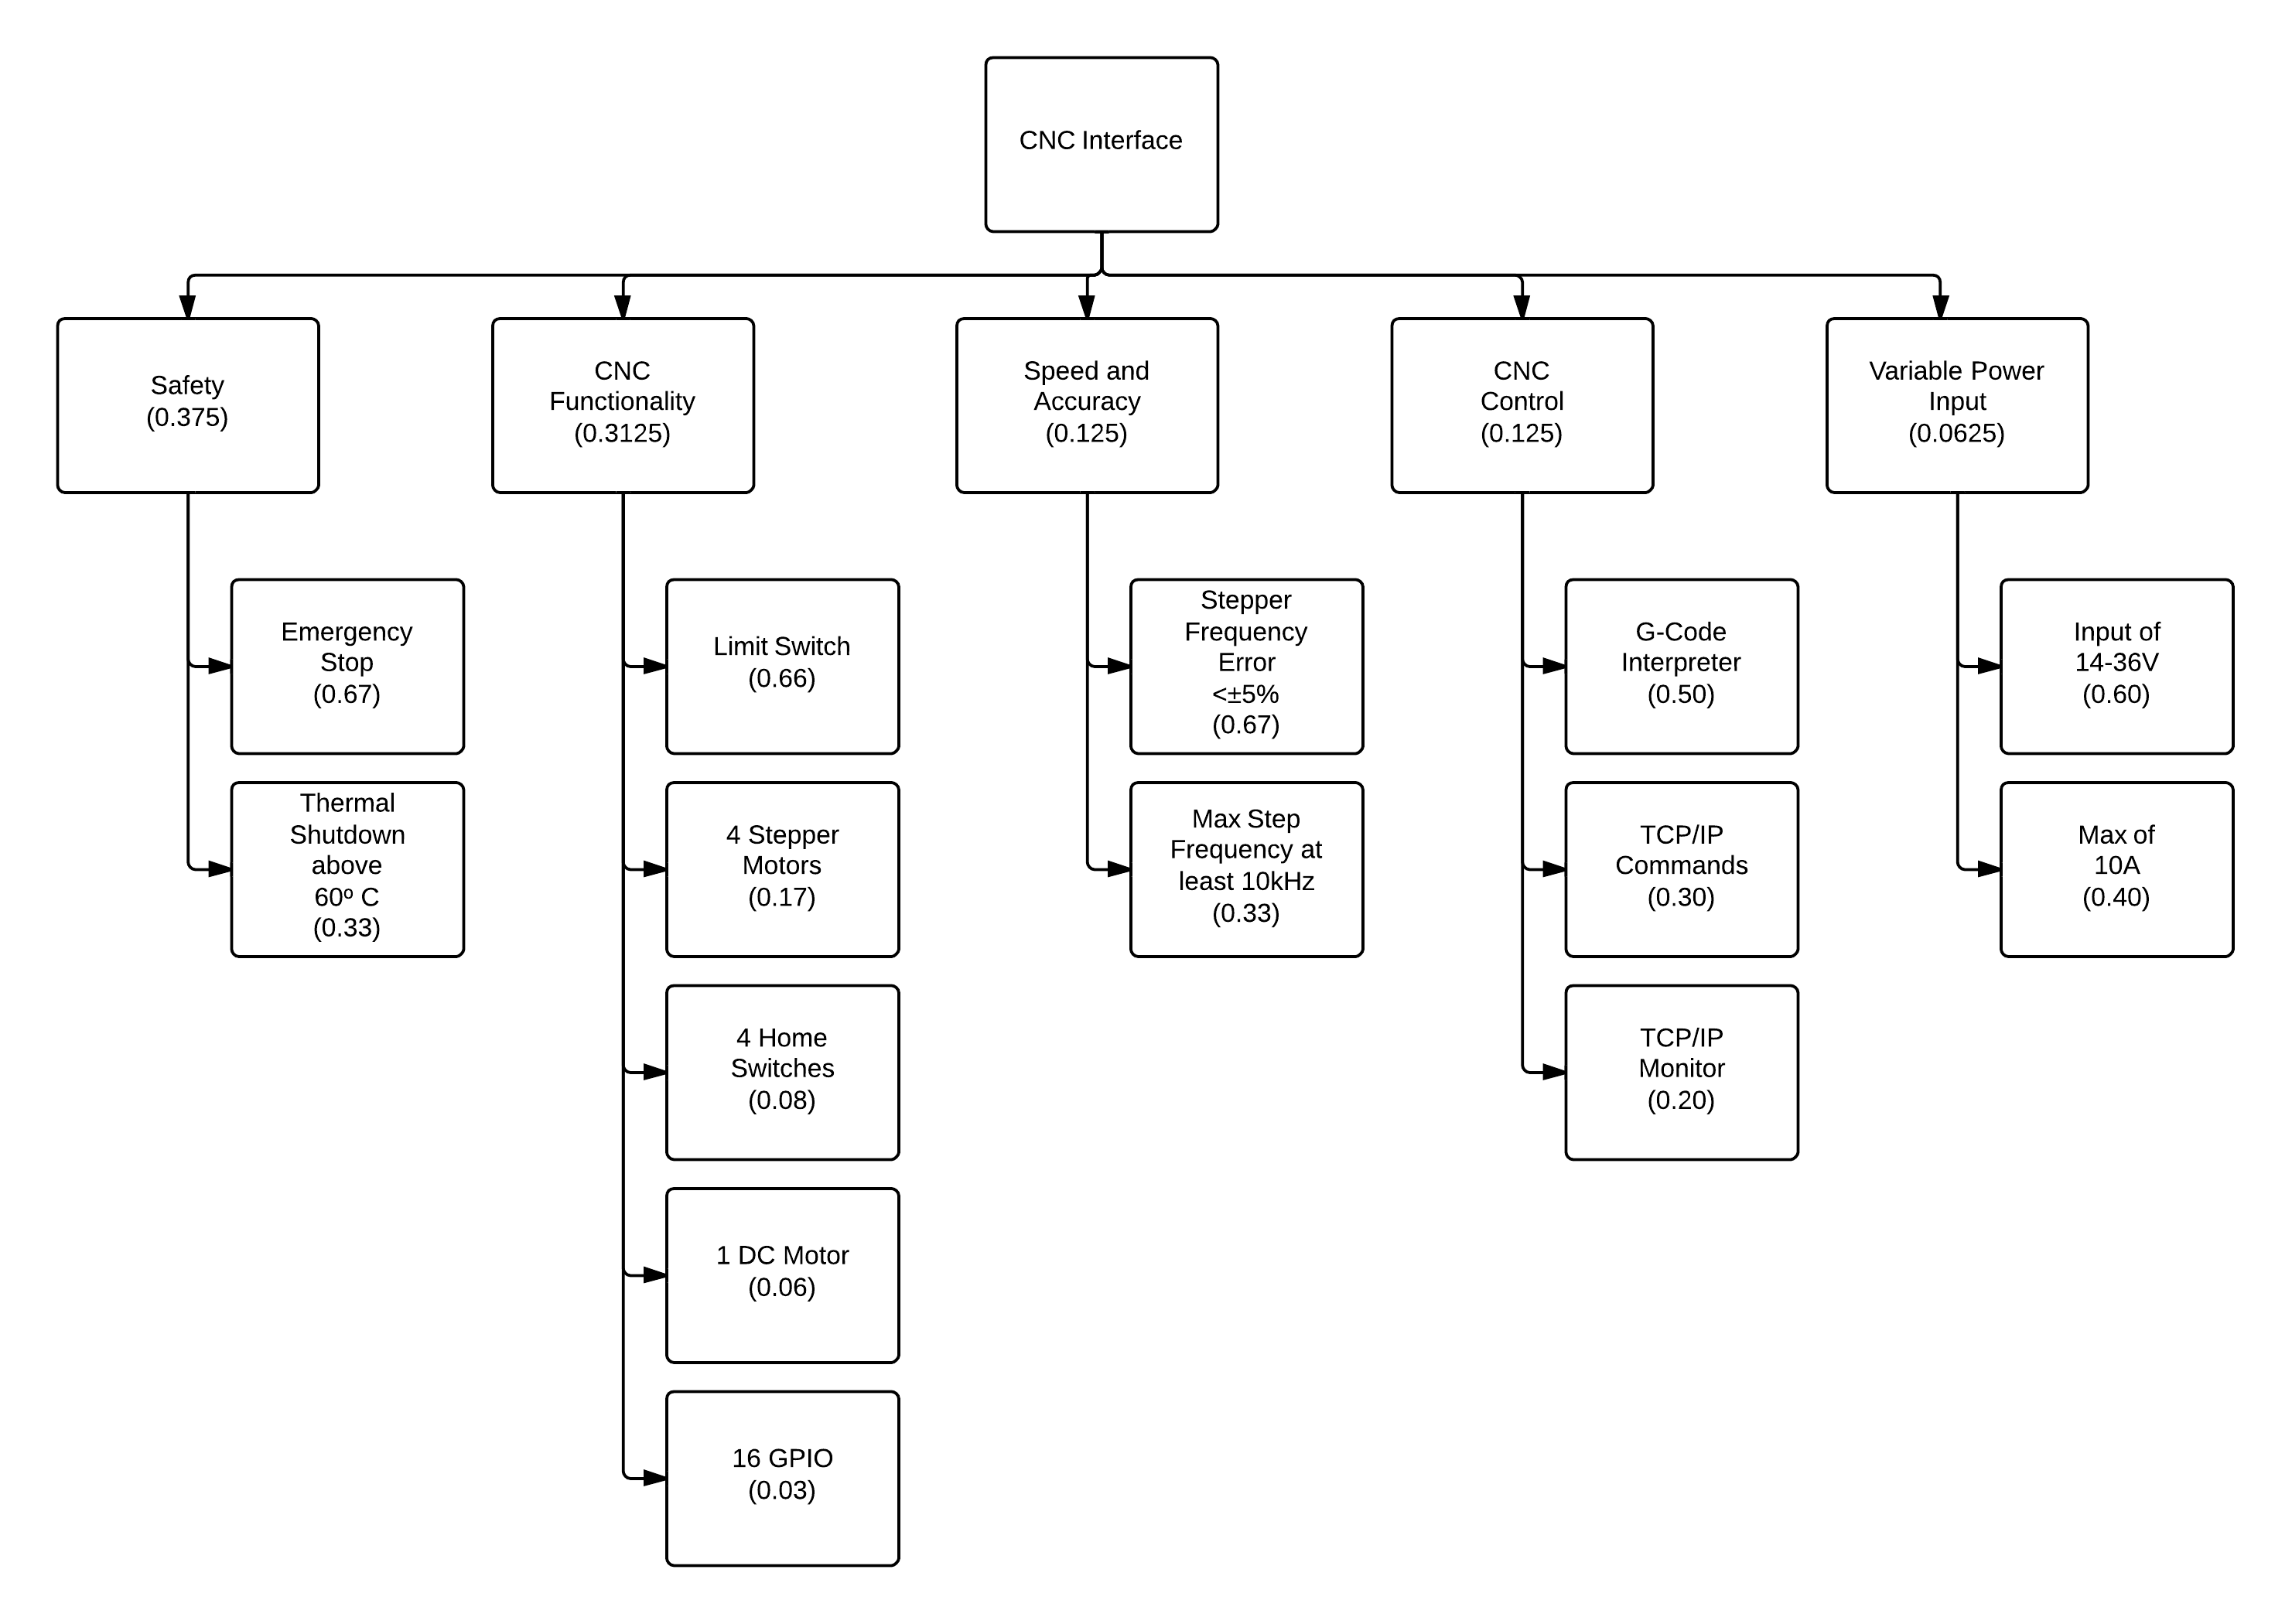
\includegraphics[width=1.0\textwidth]{otree.png}
\caption{Objective Tree}
\label{fig:o-tree}
\end{figure} 

\section{CEEN Appropriateness}
The design and execution of the CNC Interface will meet at least 7 of the 11 ABET accreditation criteria.
The design and construction will require the rigorous application of mathematics, science, and engineering for the software, hardware, mechanical, and system control. (ABET 3a).
Notably, the kinematics of the robot will require intense mathematical computations to ensure accuracy.
Experiments must be designed and conducted to ensure proper operation of components and the final result (ABET 3b).
The end result of the project will meet the needs outlined in the Background Summary (ABET 3c).
The level of success of the project will depend on how well the the team is able to cooperate and strive to achieve common goals (ABET 3d).
This project will present many engineering problems that will have to be solved (ABET 3e).
Not only must the group work towards common goals, but they must also communicate effectively (ABET 3g).
Similarly to ABET 3a, the entire project will involve the use of engineering skills that have been learned in previous coursework (ABET 3k).

The Senior Thesis Project also serves as a culmination of the CEEN curriculum. Concepts and skills learned in previous courses must be applied in the design, construction, and documentation of the project.
Courses that will be built upon in the design of the CNC Inteface are:
\begin{enumerate} \parskip2pt
	\item Microprocessor Applications
	\item Electrical \& Electronic Circuits
	\item Communication Systems
	\item Signals \& Linear Systems
	\item Digital Design \& Interface
	\item Microprocessor System Design
	\item Embedded Microcontroller Design
\end{enumerate}

\section{Revised Requirements Specification}
\textbf{Marketing Requirements}

The system will meet the following criteria:
\begin{enumerate} \parskip2pt
	
	\item be accurate in its motor control.
	\item be quickly accelerate the motors.
	\item be able to send command files through a web interface.
	\item be able to drive multiple motors.
	\item be able to handle general purpose input and output.
	\item be able to be stopped in an emergency.
	\item be able to shutdown if the system gets too hot. 
	\item be able to operate at a range of input voltages.
\end{enumerate}